\section{Evaluation}\label{sec:eval}

\begin{figure}
  \centering
  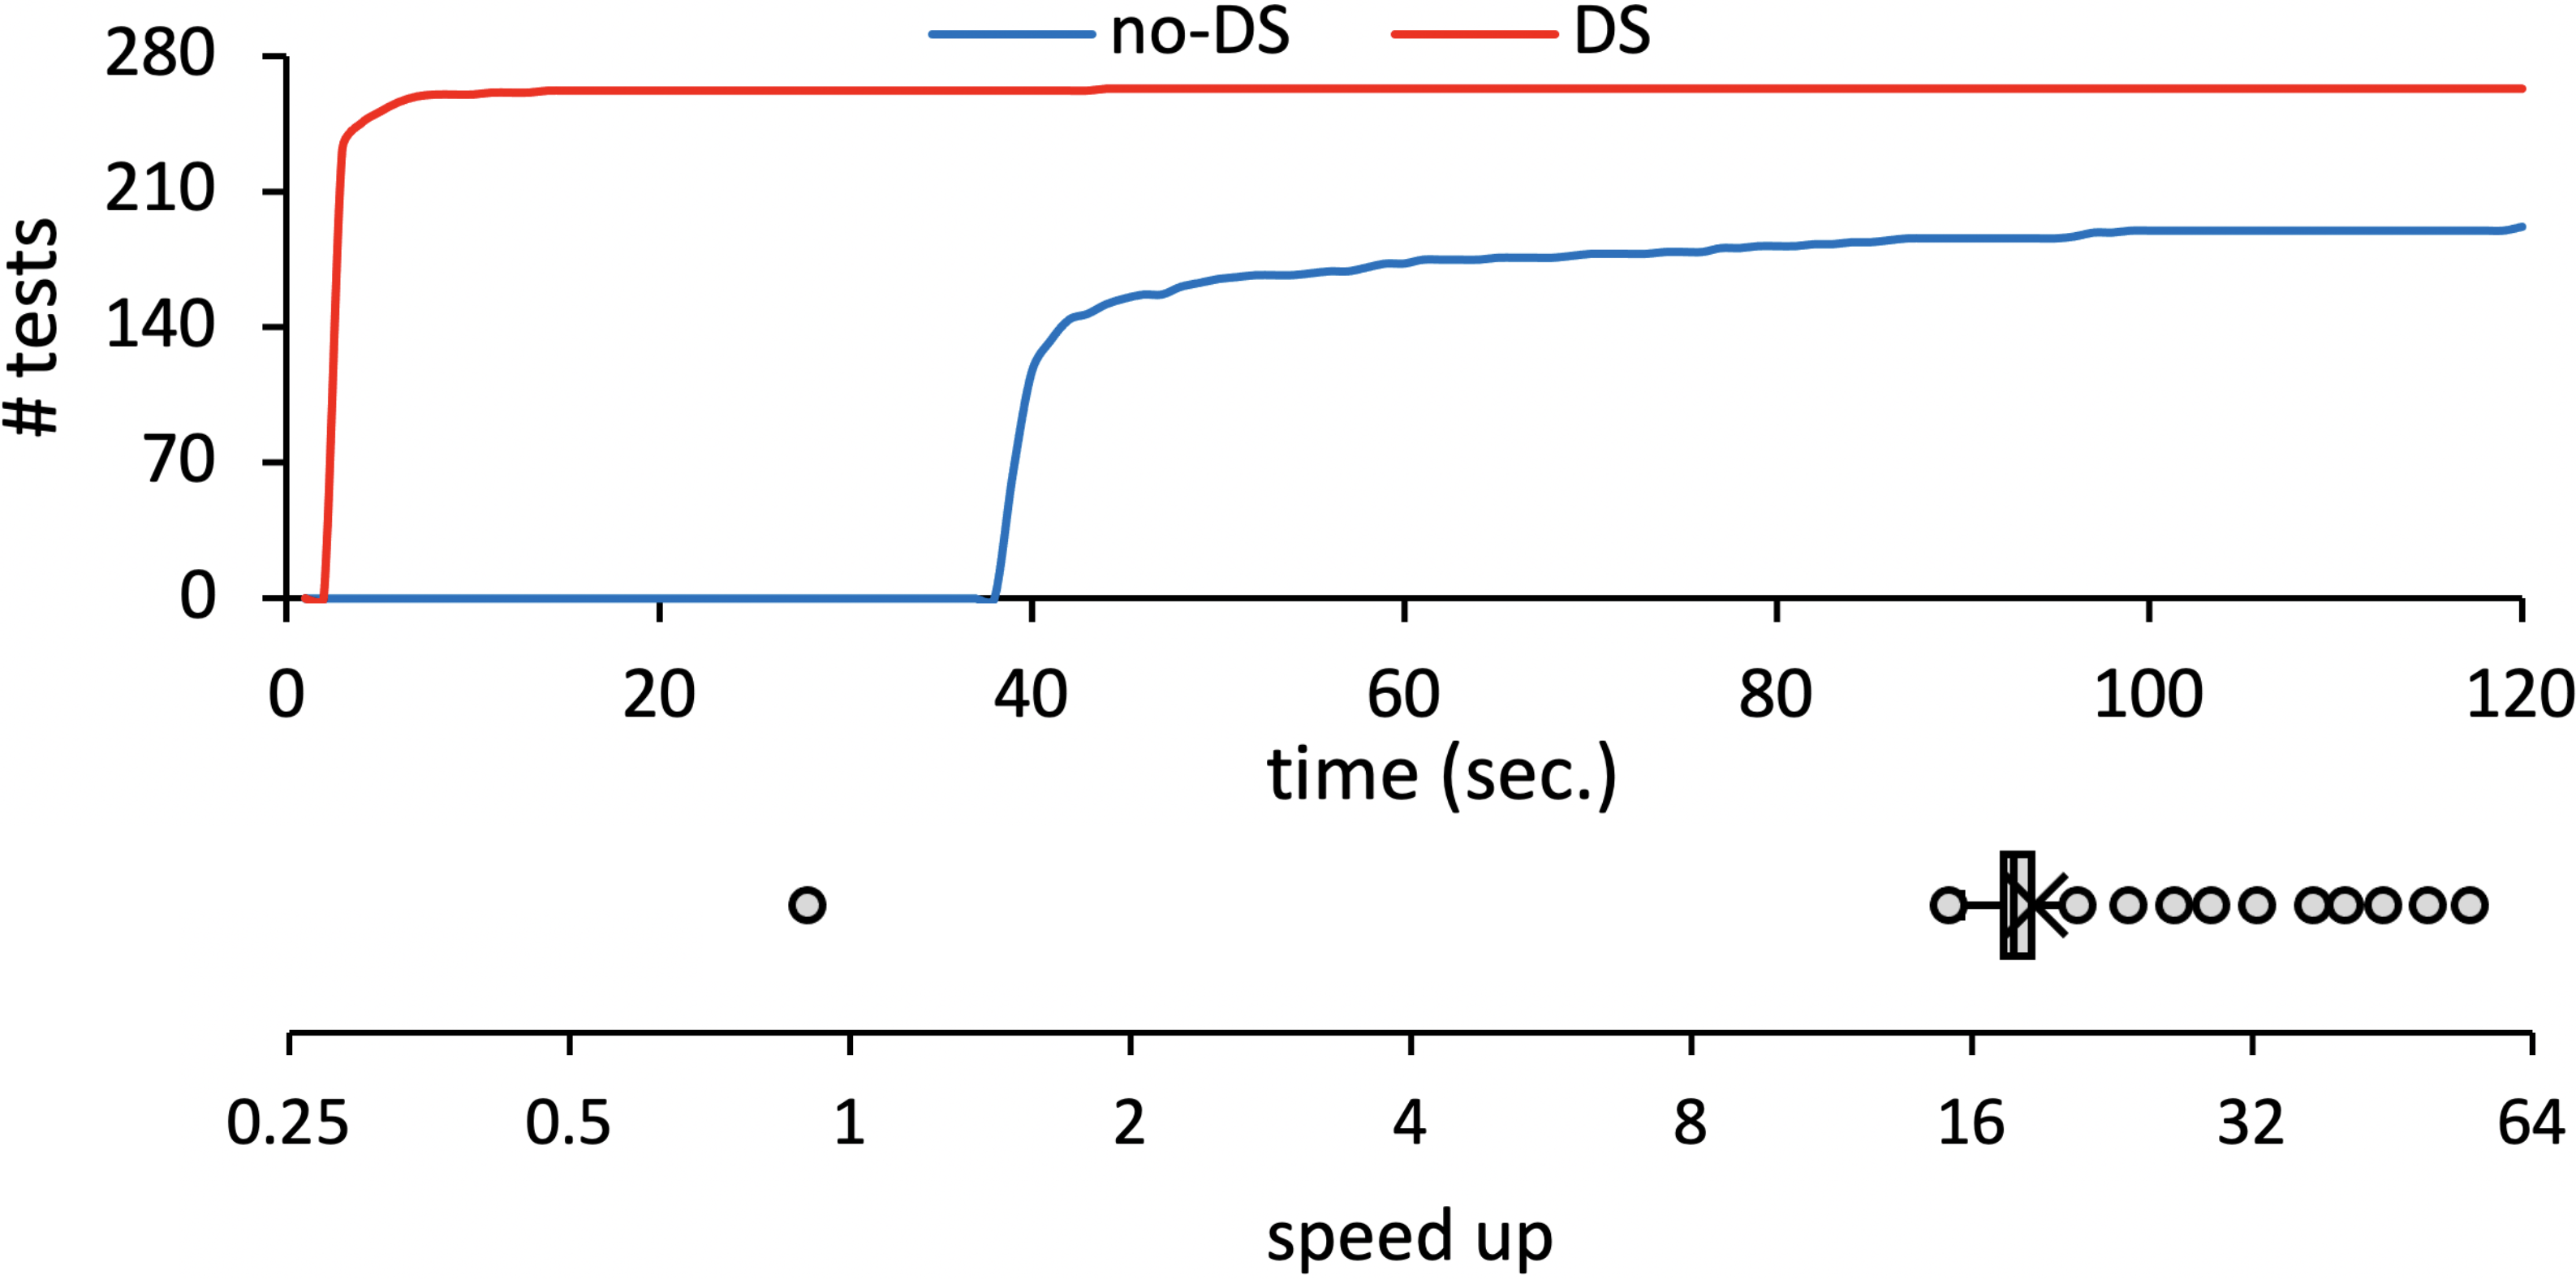
\includegraphics[width=\linewidth]{img/conc-analysis-time}
  \vspace*{-1.5em}
  \caption{Analysis time for Lodash 4 \textit{original} tests without (no-DS)
  and with (DS) the dynamic shortcut within 5 minutes.}
  \label{fig:conc-analysis-time}
  \vspace*{-1.5em}
\end{figure}

We evaluated our tool based on the following three research questions:
\begin{itemize}
\item \textbf{RQ1) Analysis Speed-up:} How much analysis time is reduced by
using dynamic shortcuts during static analysis?
\item \textbf{RQ2) Precision Improvement:} How much analysis precision is
improved by using dynamic shortcuts instead of manual modeling?
\item \textbf{RQ3) Opaque Function Coverage:} How many opaque functions are
covered by dynamic shortcuts without using manual modeling?
\end{itemize}
We selected the official 306 tests of Lodash 4
(v.4.17.20)\footnote{https://github.com/lodash/lodash/blob/4.17.20/test/test.js}
used in the motivating examples in Section~\ref{sec:motivation} as our evaluation target.
The most recent papers about JavaScript static analysis techniques~\cite{value-refinement,
value-partitioning} also used the tests to evaluate their techniques.
Among them, we filtered out \inred{37} tests that use JavaScript language
features SAFE does not support such as dynamic code generation using
\jscode{Function}, getters and setters, and browser-specific features like $\jscode{__proto__}$.
Thus, we used \inred{269} out of 306 tests for the evaluation of $\tool$.
We performed our experiments on a Ubuntu machine
equipped with 4.2GHz Quad-Core Intel Core i7 and 64GB of RAM.


\subsection{Analysis Speed-up}

\begin{figure}
  \centering
  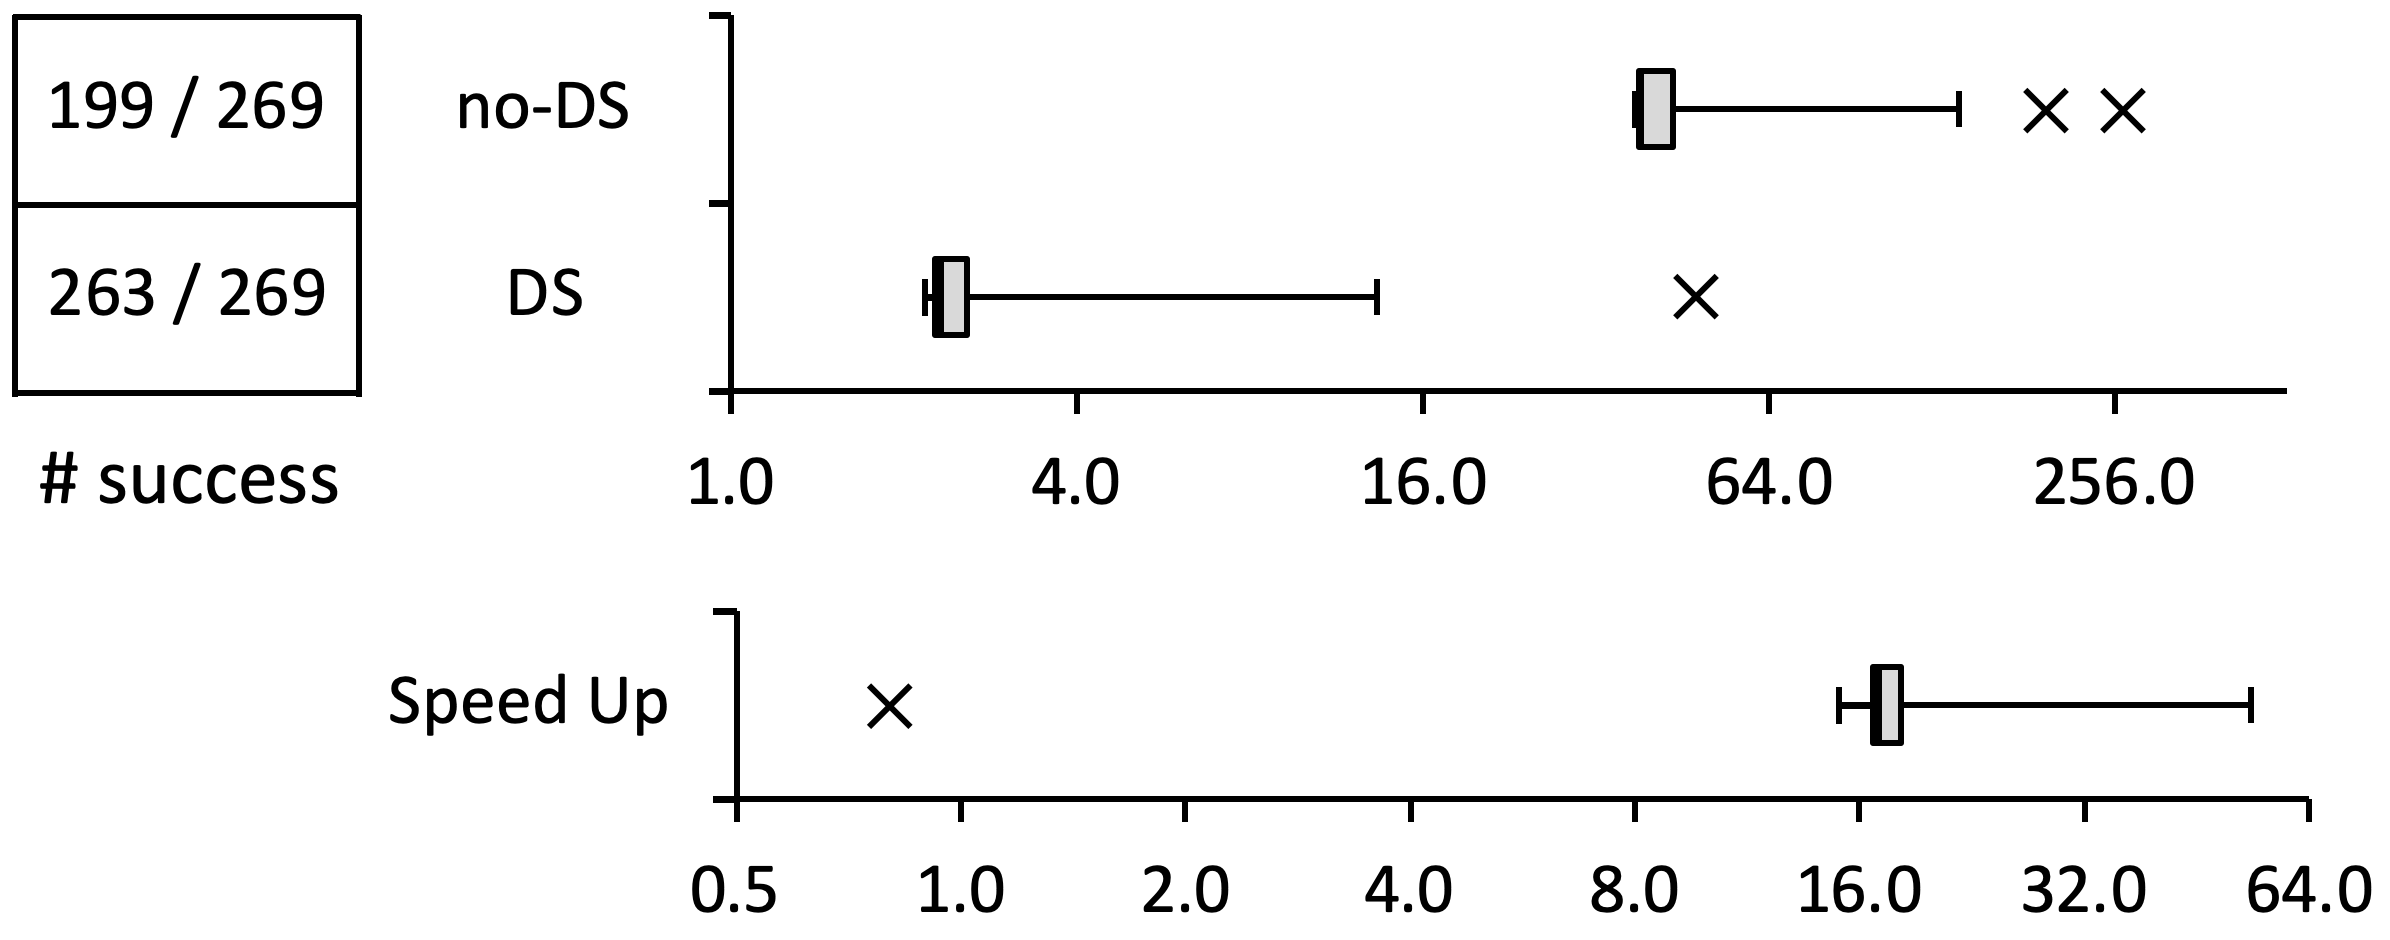
\includegraphics[width=\linewidth]{img/abs-analysis-time}
  \vspace*{-1.5em}
  \caption{Analysis time for Lodash 4 \textit{abstracted} tests without (no-DS)
  and with (DS) the dynamic shortcut within 5 minutes.}
  \label{fig:abs-analysis-time}
  \vspace*{-1.5em}
\end{figure}

To evaluate the effectiveness of using dynamic shortcuts, we performed static
analysis of \inred{269} Lodash 4 tests with and without dynamic shortcuts.
%
Figure~\ref{fig:conc-analysis-time} depicts the histogram for their analysis
time and the box plot for speed up after applying the dynamic shortcut.  While
the base analysis (no-DS) finished \inred{199} out of \inred{269} tests within 5
minutes, our tool finished all tests with the dynamic shortcut (DS).  For
\inred{199} tests analyzable by both analyses, the analysis took \inred{168.4}
seconds and \inred{12.2} seconds on average without dynamic shortcut (no-DS) and
with dynamic shortcut (DS), and the dynamic shortcut accelerates
\inred{20.16}\textsf{x} the static analysis on average.  Only for one test using
$\jscode{_.sample}$ (a Lodash 4 library that randomly samples a value from a
given array), the static analysis using dynamic shortcut had
\inred{0.81}\textsf{x} speed of the base analysis because of the frequent use of
dynamic shortcut (\inred{24} times).

Unfortunately, since most of Lodash 4 tests use concrete values instead of
non-deterministic user inputs, they could be analyzed via a few number of
dynamic shortcut.  In fact, among \inred{269} tests, \inred{262} tests analyzed
via a single usage of dynamic shortcut without using abstract semantics.
However, the arguments of library functions might include non-deterministic user
inputs in the real-world JavaScript programs.  Thus, we modified Lodash 4
official tests with abstract values to mimic the use patterns of library
functions.  We randomly selected literals and replace one of them to their
corresponding typed abstract values.  For example, if we pick a numerical
literal \jscode{42}, we modified it to the abstract numeric value
$\top_{\code{num}}$, which represents the all numerical values.  In the
remaining section, we evaluated our tool based on the \textit{original} tests
and the \textit{abstracted} tests of Lodash 4.

Also for abstracted tests, the dynamic shortcut successfully accelerates the
static analysis.  Figure~\ref{fig:abs-analysis-time} shows the analysis time for
the abstracted tests.  Among \inred{269} abstracted tests, the base analysis
(no-DS) finished \inred{82} tests within 5 minutes.  On the other hand, the
analysis using dynamic shortcut (DS) finished \inred{219} tests.  For \inred{82}
tests analyzable by both analyses, the analyses took \inred{168.4} seconds and
\inred{12.2} seconds on average without dynamic shortcut (no-DS) and with
dynamic shortcut (DS), and the dynamic shortcut accelerates
\inred{20.16}\textsf{x} the static analysis on average.

\begin{figure}
  \centering
  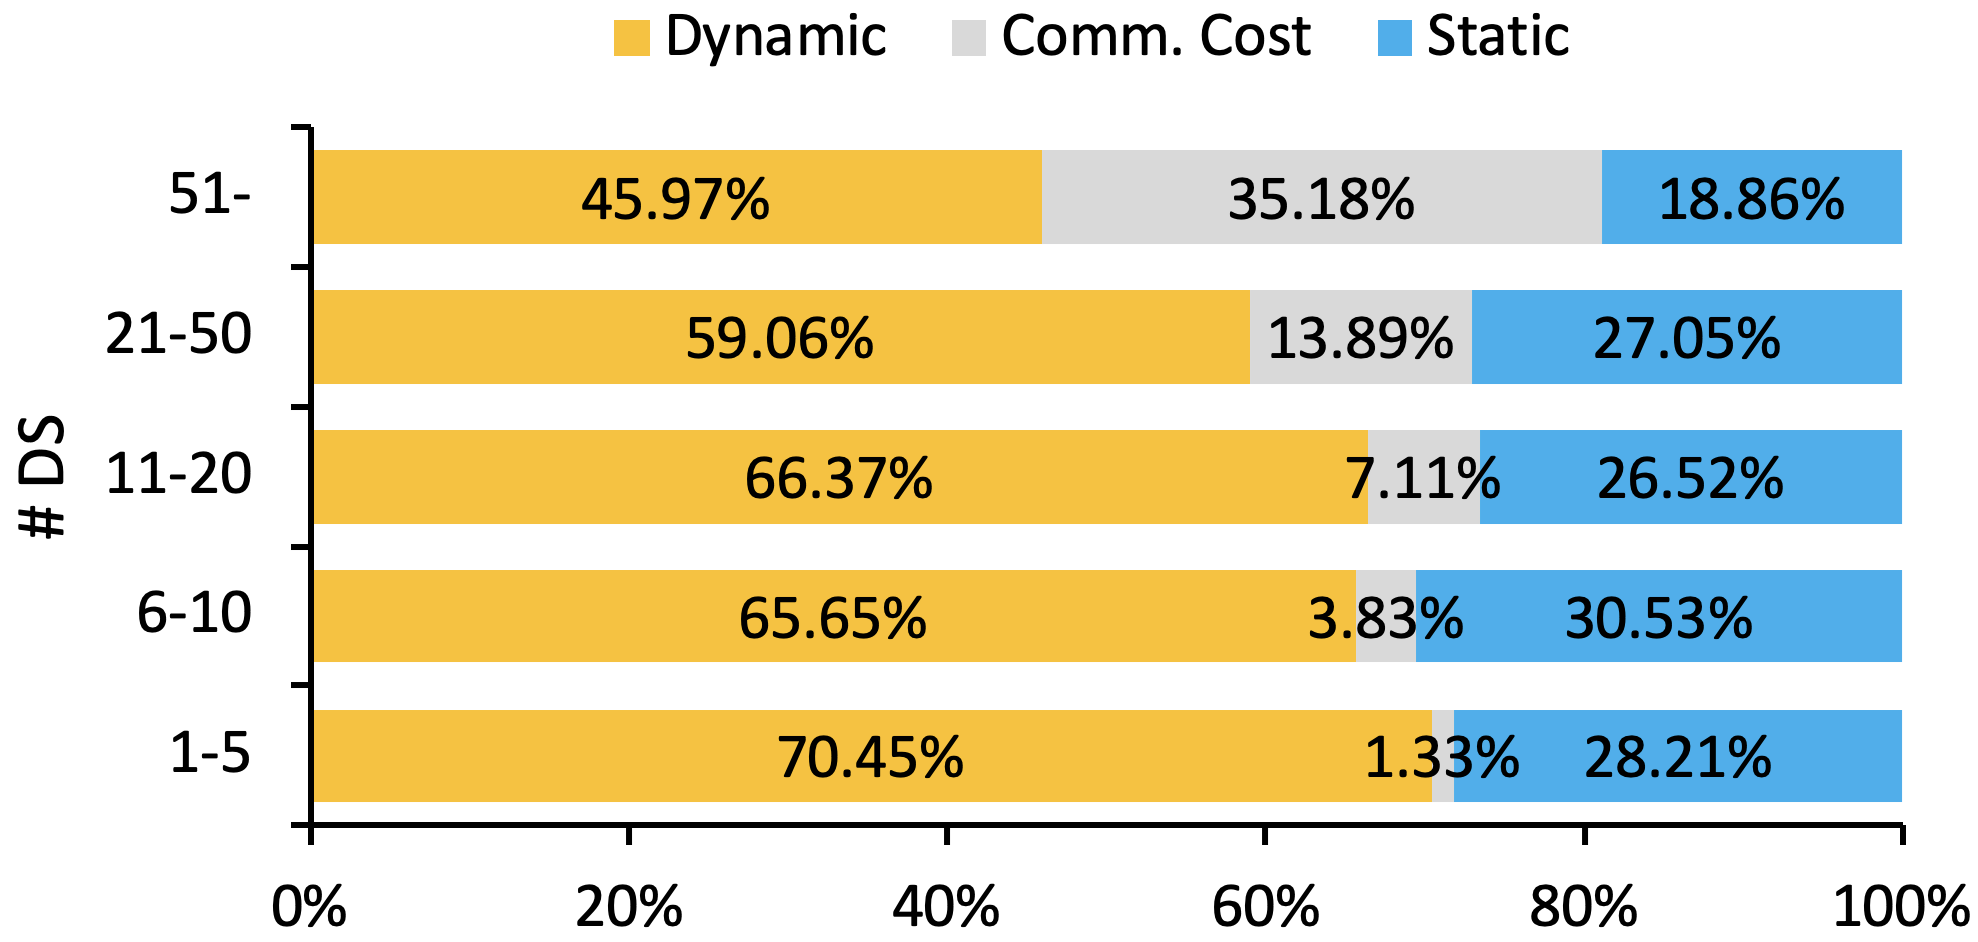
\includegraphics[width=\linewidth]{img/abs-analysis-ratio}
  \vspace*{-1.5em}
  \caption{Analysis time ratio for \inred{219} Lodash 4 \textit{abstracted}
  tests.}
  \label{fig:abs-analysis-ratio}
  \vspace*{-1.5em}
\end{figure}

Unlike Lodash 4 original tests, \inred{xx} dynamic shortcuts are invoked during
analysis for \inred{82} abstracted tests analyzable by both analyses.  We expect
the analysis time with dynamic shortcuts is propositioned to the number of
dynamic shortcuts. To communicate with the dynamic analyzer, the static analysis
should dump the current abstract state, send it to the dynamic analyzer, receive
the result from the dynamic analysis, and apply the given update information to
the abstract state.  Thus, the communication costs might increase dependent on
the number of dynamic shortcuts.  To experimentally evaluate our predictions,
we also evaluated the relationship between the number of dynamic shortcuts and
the communication costs between static and dynamic analysis.  For \inred{xx}
Lodash 4 original tests, the communication cost occupied only \inred{x.xx}\% of
total analysis.  However, for \inred{xx} abstracted tests, the communication
cost occupied \inred{xx.xx}\% in total analysis.
Figure~\ref{fig:abs-analysis-ratio} shows the detailed analysis time ratio for
\inred{82} Lodash 4 original tests.  The $x$-axis denotes the number of dynamic
shortcuts with the number of corresponding tests, and $y$-axis represents the
time ratio normalized by the total analysis time with dynamic shortcuts.  For
all \inred{82} tests, while it shows that the dynamic static analysis occupied
only \inred{x.xx}\% and \inred{27.17}\% in total analysis time, the
communication cost occupied \inred{xx.xx}\%.  If the dynamic shortcuts are
performed less than 10 times, the ratio of communication in total analysis time
is endurable because it occupied only \inred{xx.xx\%} on average.   However,
when \inred{21-30} dynamic shortcuts are performed, the communication occupied
\inred{80\%} of analysis time.  Moreover, the number of dynamic shortcuts is
more than \inred{30}, the communication time itself (DS-Comm.) is over than the
analysis time without dynamic shortcuts (no-DS).  Based on the evaluation, we
believe that it is possible to leverage dynamic shortcuts by optimizing the
communication between static and dynamic analysis.


\subsection{Precision Improvement}

\begin{figure}
  \centering
  \begin{subfigure}[t]{0.48\textwidth}
    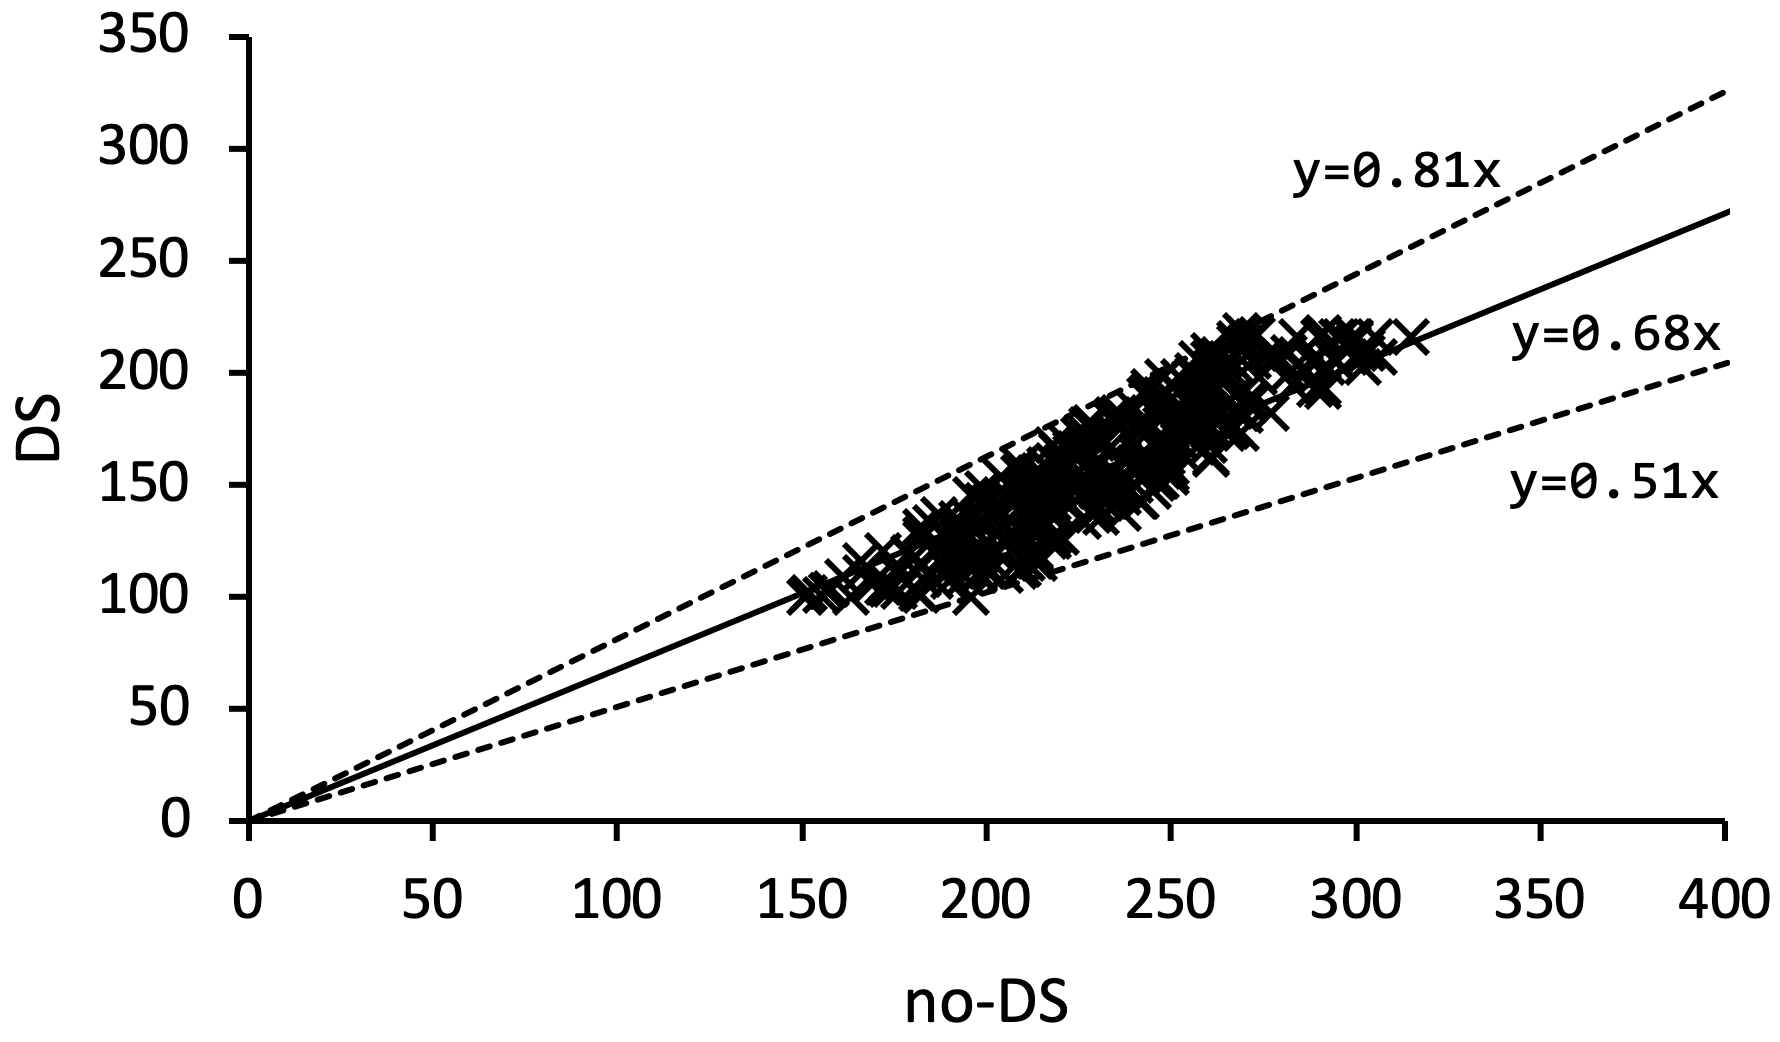
\includegraphics[width=\linewidth]{img/conc-precision}
    \vspace*{-1.5em}
    \caption{Reachable branches for \inred{xx} \textit{original} tests}
    \label{fig:precision-fail}
  \end{subfigure}
  \begin{subfigure}[t]{0.48\textwidth}
    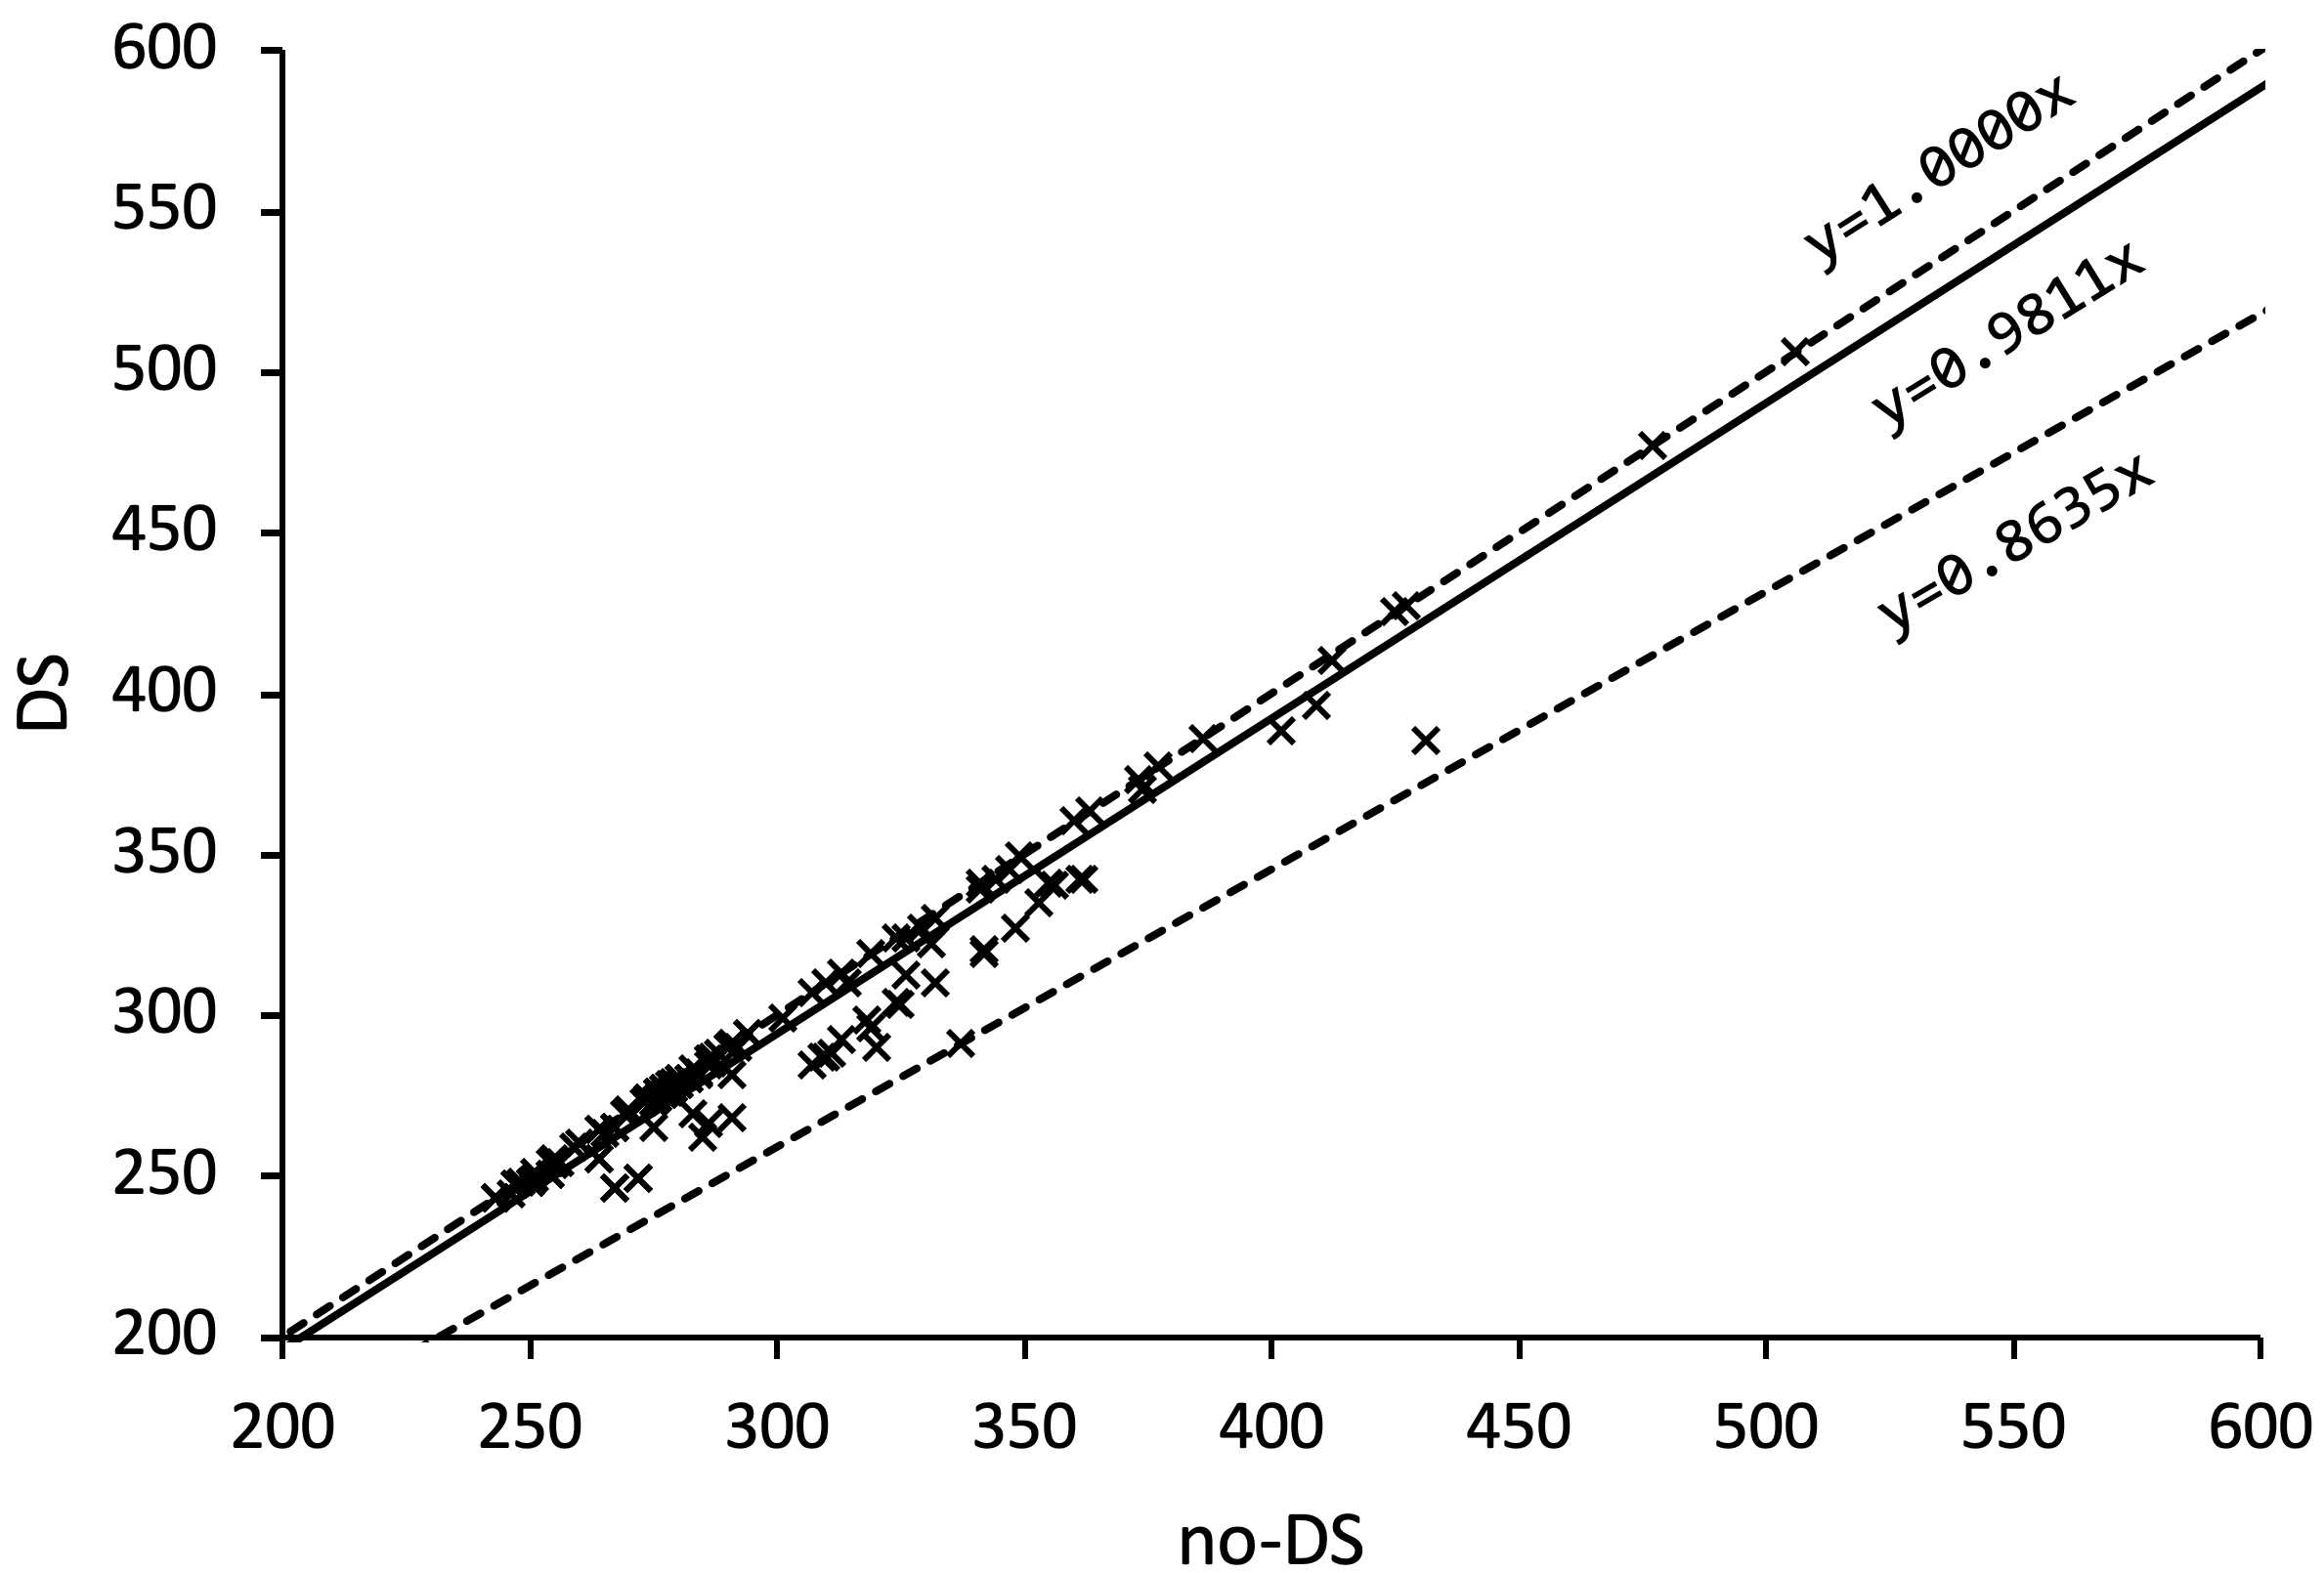
\includegraphics[width=\linewidth]{img/abs-precision}
    \vspace*{-1.5em}
    \caption{Reachable branches for \inred{82} \textit{abstracted} tests}
    \label{fig:precision-branch}
  \end{subfigure}
  \vspace*{-1em}
  \caption{The comparison of analysis precision without (no-DS) and with (DS)
  dynamic shortcut based on the branch coverage of analysis.}
  \label{fig:precision}
  \vspace*{-1.5em}
\end{figure}

\begin{table*}
  \centering
  \caption{The number of \textit{abstracted} tests using dynamic shortcut
  instead of manual modeling for each JavaScript built-in library.}
  \label{table:func-replace}
  \vspace*{-1em}
  \scriptsize
  \[
    \begin{array}{c|l|@{~}r@{~}c@{~}r@{~}r@{~}?c|l|@{~}r@{~}c@{~}r@{~}r@{~}?c|l|@{~}r@{~}c@{~}r@{~}r@{~}}

      \myhead{Object}       {Function}        {\# Replaced}

      \mysucc{2}{Boolean}   {Boolean}         {214}{214}{100} & \mydata{1}{}            {new Object}        {214}{214}{100} & \mymult{2}{Number}      {valueOf}       {214}{214}{100} \mylineff
      \mydata{1}{}          {new Boolean}     {214}{214}{100} & \mydata{1}{}            {getPrototypeOf}    {214}{214}{100} & \myname{1}{.prototype}                                  \mylinetft
      \mydata{1}{Array}     {isArray}         {214}{214}{100} & \mydata{1}{}            {create}            {214}{214}{100} & \mymult{2}{RegExp}      {toString}      {214}{214}{100} \mylinetf
      \mydata{1}{}          {toString}        { 92}{139}{ 66} & \mydata{1}{Object}      {preventExtensions} {214}{214}{100} & \myname{1}{.prototype}                                  \mylinefft
      \mydata{1}{}          {toLocaleString}  {193}{214}{ 90} & \mydata{1}{}            {isFrozen}          {214}{214}{100} & \mydata{2}{String}      {String}        {214}{214}{100} \mylinefff
      \mydata{1}{}          {concat}          {214}{214}{100} & \mydata{1}{}            {isExtensible}      {214}{214}{100} & \mydata{1}{}            {fromCharCode}  {214}{214}{100} \mylinefft
      \mydata{1}{}          {join}            {214}{214}{100} & \mydata{1}{}            {keys}              {214}{214}{100} & \mydata{1}{}            {charAt}        {214}{214}{100} \mylineftf
      \mysucc{1}{Array}     {pop}             {214}{214}{100} & \mydata{1}{Object}      {valueOf}           {214}{214}{100} & \mydata{1}{}            {charCodeAt}    {214}{214}{100} \mylinefff
      \mydata{1}{.prototype}{push}            {214}{214}{100} & \mydata{1}{.prototype}  {isPrototypeOf}     {214}{214}{100} & \mydata{1}{}            {indexOf}       {214}{214}{100} \mylineftf
      \mydata{1}{}          {slice}           {214}{214}{100} & \mydata{1}{}            {acos}              {214}{214}{100} & \mysucc{1}{}            {match}         {214}{214}{100} \mylinefff
      \mydata{1}{}          {splice}          {214}{214}{100} & \mysucc{1}{}            {atan2}             {214}{214}{100} & \mydata{1}{String}      {replace}       {214}{214}{100} \mylinefff
      \mydata{1}{}          {map}             {214}{214}{100} & \mydata{1}{}            {cos}               {214}{214}{100} & \mydata{1}{.prototype}  {splice}        {214}{214}{100} \mylinefff
      \mydata{1}{}          {reduce}          {214}{214}{100} & \mydata{1}{Math}        {exp}               {214}{214}{100} & \mydata{1}{}            {split}         {214}{214}{100} \mylinetff
      \mysucc{1}{global}    {eval}            {214}{214}{100} & \mydata{1}{}            {floor}             {214}{214}{100} & \mysucc{1}{}            {substring}     {214}{214}{100} \mylinetff
      \mydata{1}{}          {new Date}        {214}{214}{100} & \mydata{1}{}            {max}               {214}{214}{100} & \mydata{1}{}            {toLowerCase}   {214}{214}{100} \mylinefff
      \mydata{1}{Date}      {parse}           {214}{214}{100} & \mydata{1}{}            {min}               {214}{214}{100} & \mydata{1}{}            {toUpperCase}   {214}{214}{100} \mylinef
      \mydata{1}{}          {now}             {214}{214}{100}
    \end{array}
  \]
  \vspace*{-1em}
\end{table*}

To evaluate the precision improvement of dynamic shortcut, we used the number of
branches covered by analysis to measure the precision of the analysis results.
One of the most popular application of static analysis is dead code elimination
by using the result of reachability analysis.  To acquire smaller codes, precise
reachability analysis is required.  Thus, we decided to measure the analysis
precision based on the number of branches covered by analysis.  The high
branch coverage denotes the low analysis precision, and low branch coverage
denotes the high precision.  Figure~\ref{fig:precision} depicts the comparison of
the number of covered branches without (no-DS) and with (DS) dynamic shortcuts
for \inred{xx} original tests and \inred{xx} abstracted tests.

For \inred{xx} both analyzable original tests, Figure~\ref{fig:conc-precision}
shows the number of branches covered by analysis.  The $x$- and $y$-axis denote
the analysis without (no-DS) and with (DS) dynamic shortcuts and each $\times$
mark denotes each test.  The top and bottom dotted lines denote the worst and
best precision improvement, and the middle solid line denotes the average
improvement.  Thus, dynamic shortcuts successfully reduced the number of
branches at least \inred{1.00}\textsc{x}, at most \inred{0.54}\textsc{x}, and
\inred{0.92}x on average.  For abstracted tests, we evaluated \inred{xx} tests
analyzable by both analyses.  Figure~\ref{fig:precision-branch} depicts the
results of experiments for abstracted tests and it shows that dynamic shortcuts
also successfully cuts down the number of covered branches at least
\inred{0.81}\textsc{x}, at most \inred{0.51}\textsc{x}, and
\inred{0.68}\textsc{x} on average.


\subsection{Opaque Function Coverage}

The dynamic shortcut does not only improve performance or precision of analysis
but also reduce the effort to model the behavior of opaque functions.
JavaScript programs often use JavaScript built-in libraries or host-dependent
functions but they are opaque codes; it means that they are executable but
written in a different programming languages.  A typical solution is to
manually model their behaviors to statically analyze for JavaScript programs
using such functions.  The dynamic shortcut can reduce such efforts if some
opaque functions are analyzed by only dynamic analysis instead of static
analysis.

Table~\ref{table:func-replace} describes the dynamic shortcut effectively lessen
the burden of manual modeling for JavaScript built-in functions.  For Lodash 4
\inred{xx} original tests and \inred{xx} abstracted tests, we measured the
number of tests using only dynamic shortcut instead of manual modeling for each
JavaScript built-in library.  For each raw, \textbf{Object} column denotes the
built-in object, \textbf{Function} function name, \textbf{\# Replaced} the
number of tests successfully replacing the modeling via dynamic shortcut with
the total number of tests using the target function.  For example, the fourth
row in the left side describes that \jscode{Array.prototype.toString} is used in
\inred{139} original tests and \inred{xxx} abstracted tests. Amogn them,
\inred{44} original tests \inred{xx} abstracted tests are successfully analyzed
by dynamic shortcuts instead of using the modeling of
\jscode{Array.prototype.toString}.

Moreover, several built-in functions are analyzed by only dynamic shortcuts in
all tests.  Among \inred{49} JavaScript built-in functions, \inred{xx} and
\inred{xx} functions are analyzed by only dynamic shortcut instead of manual
modeling for all original or all abstracted tests.  Each cell colored by
\inred{yellow} describes fully replaceable cases in
Table~\ref{table:func-replace}.
